\section{Case Study 1: Spatial SIR Model} %(First Encounter)
\label{sec:cs_sir}

Our first case study is the SIR model which is a very well studied and understood compartment model from epidemiology \cite{kermack_contribution_1927} which allows to simulate the dynamics of an infectious disease like influenza, tuberculosis, chicken pox, rubella and measles spreading through a population \cite{enns_its_2010}.

In it, people in a population of size $N$ can be in either one of three states \textit{Susceptible}, \textit{Infected} or \textit{Recovered} at a particular time, where it is assumed that initially there is at least one infected person in the population. People interact \textit{on average} with a given rate of $\beta$ other people per time-unit and become infected with a given probability $\gamma$ when interacting with an infected person. When infected, a person recovers \textit{on average} after $\delta$ time-units and is then immune to further infections. An interaction between infected persons does not lead to re-infection, thus these interactions are ignored in this model. 

We followed in our agent-based implementation of the SIR model the work \cite{macal_agent-based_2010} but extended it by placing the agents on a discrete 2D grid using a Moore (8 surrounding cells) neighbourhood \cite{thaler_pure_2019}. A visualisation can be seen in Figure \ref{fig:vis_sir}.

It is important to note that due to the continuous-time nature of the SIR model, our implementation follows the time-driven \cite{meyer_event-driven_2014} approach. This requires us to sample the system with very small $\Delta t$, which means that we have comparatively few writes to the shared environment which will become important when discussing the performance results.

\begin{figure}
	\centering
	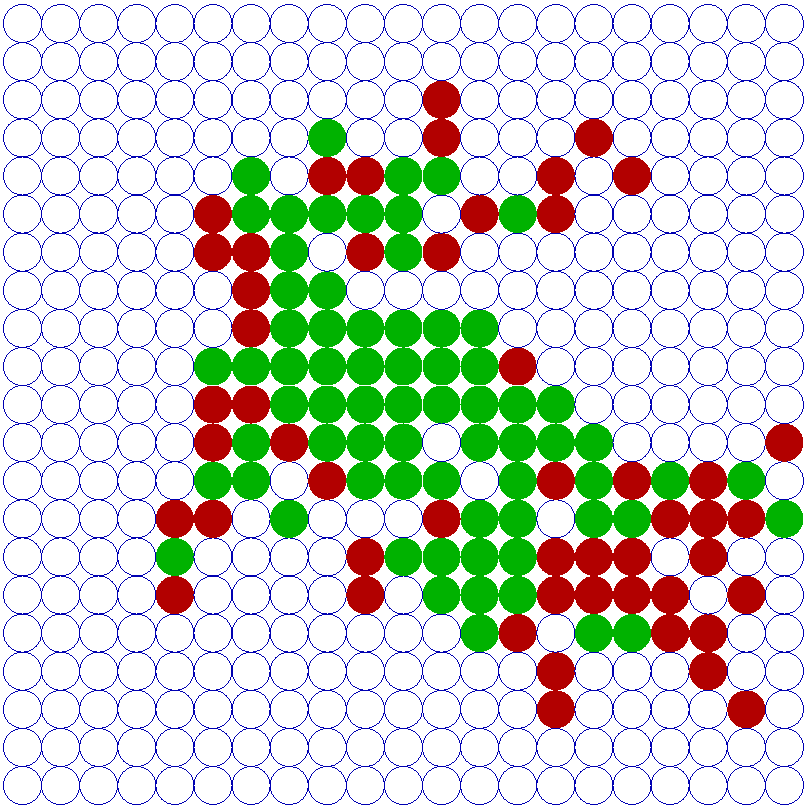
\includegraphics[width=0.4\textwidth, angle=0]{./fig/sir/vis/SIR_Dunai_dt001_environment.png}
	\caption{Simulating the spatial SIR model with a Moore neighbourhood, a single infected agent at the center, contact rate $\beta = \frac{1}{5}$, infection probability $\gamma = 0.05$ and illness duration $\delta = 15$ . Infected agents are indicated by red circles, recovered agents by green ones. The susceptible agents are rendered as blue hollow circles for better contrast.}
	\label{fig:vis_sir}
\end{figure}

\subsection{Experiment Design}
In this case study we compare the performance of the following implementations under varying numbers of CPU cores and agent numbers \footnote{The code is freely available at \url{https://github.com/thalerjonathan/phd/tree/master/public/stmabs/code/SIR}}:

\begin{enumerate}
	\item Sequential - This is the original implementation as discussed in \cite{thaler_pure_2019} where the discrete 2D grid is shared amongst all agents as read-only data and the agents are executed sequentially within the main thread without any concurrency.
	\item STM - This is the same implementation as the \textit{Sequential} but agents run now in the STM context and have access to the discrete 2D grid through a transactional variable \textit{TVar}. This means that the agents now communicate indirectly by reads and writes through the \textit{TVar}.
	\item Lock-Based - This is exactly the same implementation as the \textit{STM} one, but instead of running in the STM context, the agents now run in IO context. They share the discrete 2D grid using a global reference and have access to a lock to synchronise access to it.
	\item RePast - To have an idea where the functional implementation is performance-wise compared to the established object-oriented methods, we implemented a Java version of the SIR model using RePast \cite{north_complex_2013} with the state-chart feature. This implementation cannot run on multiple cores concurrently but gives a good estimate of the single core performance of imperative approaches. Although there exists a RePast High Performance Computing library for implementing large-scale distributed simulations in C++, we leave this for further research as an implementation and comparison is out of the scope of this paper.
\end{enumerate}

Each experiment was run until $t = 100$ and stepped using $\Delta t = 0.1$ except in RePast for which we don't have access to the underlying implementation of the state-chart and left it as it is. For each experiment we conducted 8 runs on our machine (see Table \ref{tab:machine_specs}) under no additional work-load and report the mean. Further, we checked the visual outputs and the dynamics and they look qualitatively the same as the reference \textit{Sequential} implementation \cite{thaler_pure_2019} - we could have used more rigour and properly validated the implementations against the formal specification using tests but this was beyond the scope of this paper. In the experiments we varied the number of agents (grid size) as well as the number of cores when running concurrently (through run-time system arguments) - the numbers are always indicated clearly. %For varying the number of cores we compiled the executable using the tool \textit{stack} with the \textit{threaded} option and executed it with \textit{stack} using the +RTS -Nx option where x indicates the number of cores. 

\begin{table}
	\centering
	\begin{tabular}{ c || c }
		OS & Fedora 28 64-bit \\ \hline
		RAM & 16 GByte \\ \hline
		CPU & Intel Quad Core i5-4670K @ 3.4GHz (4th Gen.) \\ \hline
		HD & 250Gbyte SSD \\ \hline
		Haskell & GHC 8.2.2 \\ \hline
		Java & OpenJDK 1.8.0 \\ \hline
		RePast & 2.5.0.a
	\end{tabular}
	
	\caption{Machine and Software Specs for all experiments}
	\label{tab:machine_specs}
\end{table}

\subsection{Constant Grid Size, Varying Cores}
In this experiment we held the grid size constant to 51 x 51 (2,601 agents) and varied the cores where possible. The results are reported in Table \ref{tab:constgrid_varyingcores}.

\begin{table}
	\centering
	\begin{tabular}{cc|c}
		\multicolumn{1}{ c||  }{\multirow{2}{*}{} } &
		\multicolumn{1}{ |c| }{Cores} & Duration       \\ \hline \hline 
		
		\multicolumn{1}{ c||  }{\multirow{1}{*}{Sequential} } &
		\multicolumn{1}{ |c| }{1} & 72.5      \\ \hline \hline 
		
		\multicolumn{1}{ c||  }{\multirow{4}{*}{Lock-Based} } &
		\multicolumn{1}{ |c| }{1} & 60.6       \\ \cline{2-3}
		\multicolumn{1}{ c||  }{}                       &
		\multicolumn{1}{ |c| }{2} & 42.8    \\ \cline{2-3}
		\multicolumn{1}{ c||  }{}                       &
		\multicolumn{1}{ |c| }{3} & 38.6    \\ \cline{2-3}
		\multicolumn{1}{ c||  }{}                       &
		\multicolumn{1}{ |c| }{4} & 41.6    \\ \hline \hline 
		
		\multicolumn{1}{ c||  }{\multirow{4}{*}{STM} } &
		\multicolumn{1}{ |c| }{1} & 53.2       \\ \cline{2-3}
		\multicolumn{1}{ c||  }{}                       &
		\multicolumn{1}{ |c| }{2} & 27.8    \\ \cline{2-3}
		\multicolumn{1}{ c||  }{}                       &
		\multicolumn{1}{ |c| }{3} & 21.8    \\ \cline{2-3}
		\multicolumn{1}{ c||  }{}                       &
		\multicolumn{1}{ |c| }{4} & 20.8    \\ \hline \hline 
		
		\multicolumn{1}{ c||  }{\multirow{1}{*}{RePast} } &
		\multicolumn{1}{ |c| }{1} & \textbf{10.8}      \\ \hline \hline 
	\end{tabular}
  	
  	\caption{Experiments on 51x51 (2,601 agents) grid with varying number of cores.}
	\label{tab:constgrid_varyingcores}
\end{table}

Comparing the performance and scaling to multiple cores of the \textit{STM} and \textit{Lock-Based} implementations shows that the \textit{STM} implementation significantly outperforms the \textit{Lock-Based} one and scales better to multiple cores. The \textit{Lock-Based} implementation performs best with 3 cores and shows slightly worse performance on 4 cores as can be s een in Figure \ref{fig:core_duration_stm_io}. This is no surprise because the more cores are running at the same time, the more contention for the lock, thus the more likely synchronisation happening, resulting in higher potential for reduced performance. This is not an issue in \textit{STM} because no locks are taken in advance. 

What comes a bit as a surprise is, that the single core RePast implementation significantly outperforms \textit{all} other implementations, even when they run on multiple cores and even with RePast doing complex visualisation in addition (something the functional implementations don't do). When looking at benchmarks \footnote{\url{https://benchmarksgame-team.pages.debian.net/benchmarksgame/faster/haskell.html}} comparing Haskell to Java, C and C++, Haskell is significantly outperformed in most of the cases. This is a strong indication that Haskell is in general not as fast as Java, C or C++. %Although there exist advanced techniques where Haskell can approach a performance like C \cite{kqr_competing_2017} we don't use them here as often this comes at the cost of more complex features, some of them not part of the language standard, more complex code and ultimately requires lots of experience .
Also, we build on the concepts developed in \cite{thaler_pure_2019} to implement our ABS which make heavy use of Functional Reactive Programming, which can be substantially slower than imperative approaches \cite{nilsson_functional_2002, hudak_arrows_2003}. 

\begin{figure}
	\centering
	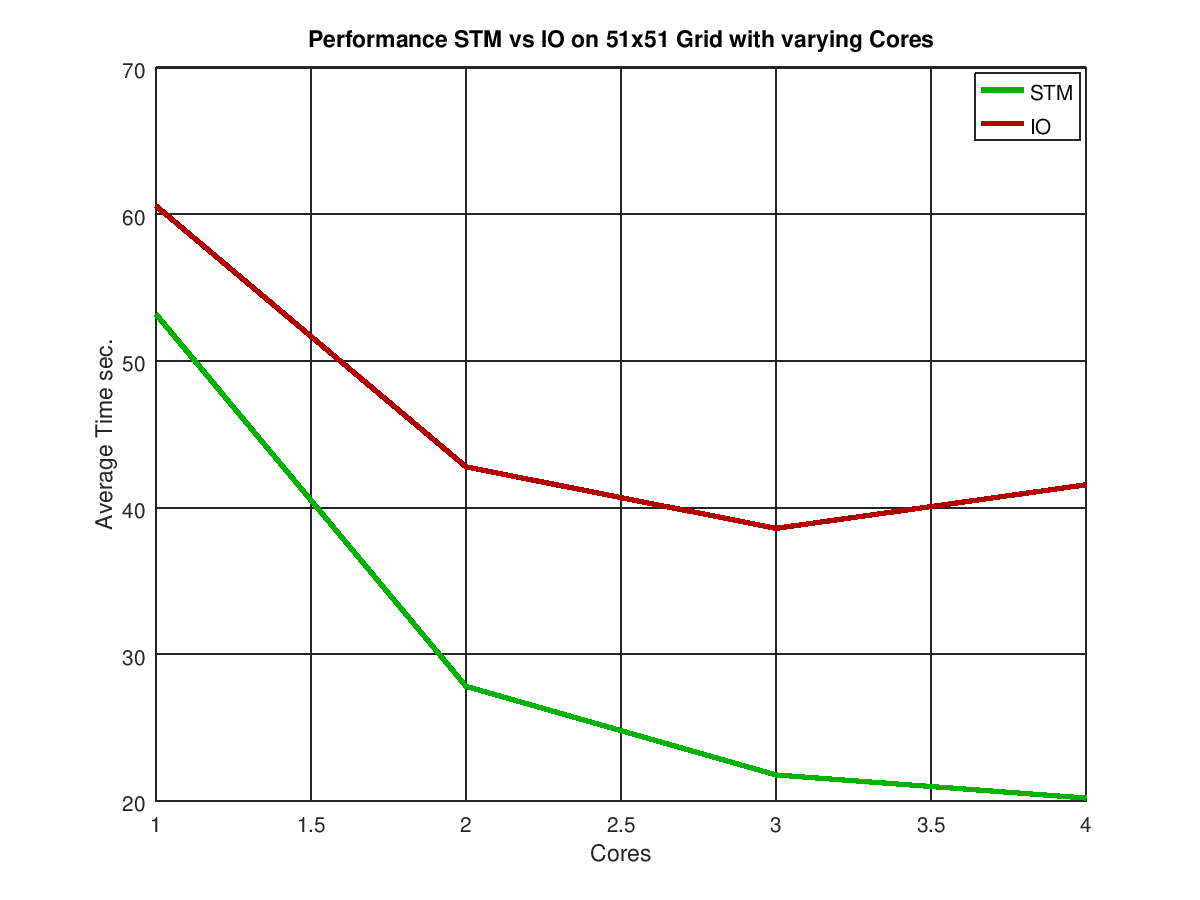
\includegraphics[width=0.6\textwidth, angle=0]{./fig/sir/core_duration_stm_io.png}
	\caption{Comparison of performance and scaling on multiple cores of STM vs. Lock-Based. Note that the Lock-Based implementation performs worse on 4 than on 3 cores due to lock-contention.}
	\label{fig:core_duration_stm_io}
\end{figure}

\subsection{Varying Grid Size, Constant Cores}
In this experiment we varied the grid size and used constantly 4 cores. Because in the previous experiment \textit{Lock-Based} performed best on 3 cores, we additionally ran Lock-Based on 3 cores as well. Note that the RePast experiments all ran on a single (1) core and were conducted to have a rough estimate where the functional approach is in comparison to the imperative. The results are reported in Table \ref{tab:varyinggrid_constcores} and plotted in Figure \ref{fig:varyinggrid_constcores}.

\begin{table}
	\centering
  	\begin{tabular}{ c || c | c | c | c }
        Grid-Size          & STM              & Lock-Based (4 cores) & Lock-Based (3 cores) & RePast (1 core) \\ \hline \hline 
   		51 x 51 (2,601)    & 20.2             & 41.9                 & 38.6                 & \textbf{10.8}   \\ \hline
   		101 x 101 (1,0201) & \textbf{74.5}    & 170.5                & 171.6                & 107.40          \\ \hline
   		151 x 151 (22,801) & \textbf{168.5}   & 376.9                & 404.1                & 464.1           \\ \hline
   		201 x 201 (40,401) & \textbf{302.4}   & 672.0                & 720.6                & 1,227.7         \\ \hline
   		251 x 251 (63,001) & \textbf{495.7}   & 1,027.3              & 1,117.2              & 3,283.6         \\ \hline \hline
  	\end{tabular}

  	\caption{Performance on varying grid sizes.}
	\label{tab:varyinggrid_constcores}
\end{table}

It is clear that the \textit{STM} implementation outperforms the \textit{Lock-Based} implementation by a substantial factor. Surprisingly, the \textit{Lock-Based} implementation on 4 core scales just slightly better with increasing agents number than on 3 cores, something we wouldn't have anticipated based on the results seen in Table \ref{tab:constgrid_varyingcores}. Also  while on a 51x51 grid the single (1) core Java \textit{RePast} version outperforms the 4 core Haskell \textit{STM} version by a factor of 2. The figure is inverted on a 251x251 grid where the 4 core Haskell \textit{STM} version outperforms the single core Java \textit{Repast} version by a factor of 6. This might not be entirely surprising because we compare single (1) core against multi-core performance - still the scaling is indeed impressive and we would not have anticipated an increase of factor 6. %The RePast implementation shows an exponential increase of computation time whereas the other implementations scale linearly which we attribute to the use of multi-cores.

\begin{figure}
\begin{center}
	\begin{tabular}{c c}
		\begin{subfigure}[b]{0.5\textwidth}
			\centering
			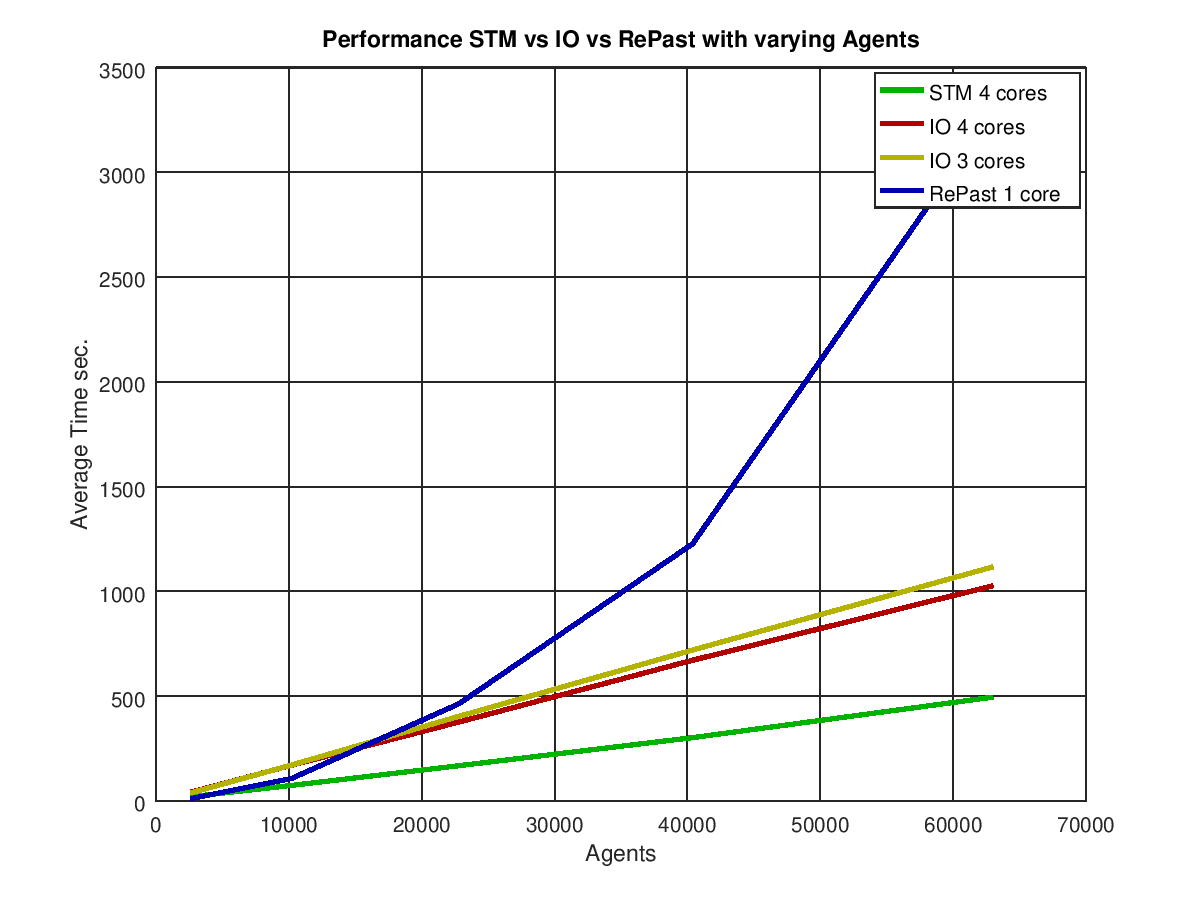
\includegraphics[width=1\textwidth, angle=0]{./fig/sir/stm_io_repast_varyinggrid_performance.png}
			\caption{Normal Scale}
		\end{subfigure}
    	&
		\begin{subfigure}[b]{0.5\textwidth}
			\centering
			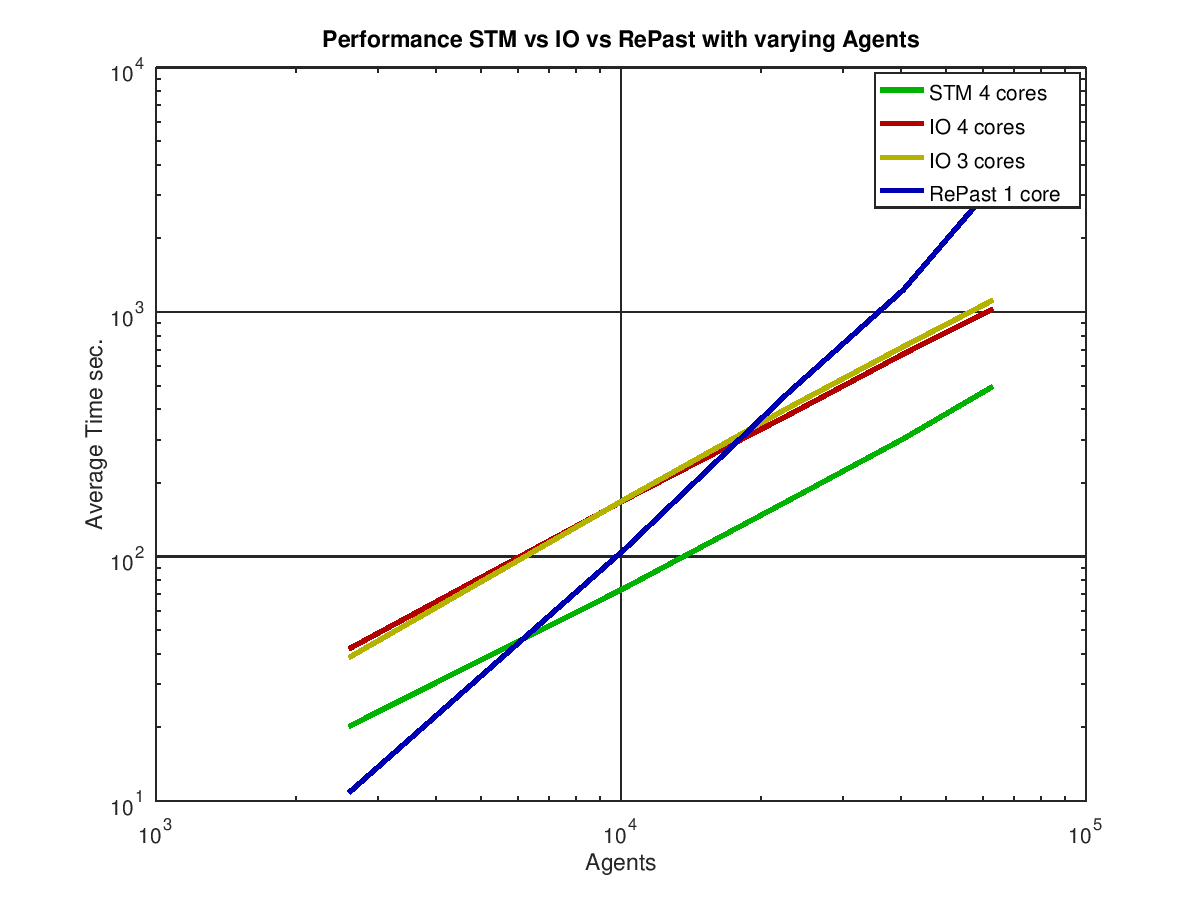
\includegraphics[width=1\textwidth, angle=0]{./fig/sir/stm_io_repast_varyinggrid_performance_loglog.png}
			\caption{Logarithmic scale on both axes}
		\end{subfigure}
    \end{tabular}
	\caption{Performance on varying grid sizes.}
	\label{fig:varyinggrid_constcores}
\end{center}
\end{figure}

\subsection{Retries}
Of very much interest when using STM is the retry-ratio, which obviously depends highly on the read-write patterns of the respective model. We used the \textit{stm-stats} library to record statistics of commits, retries and the ratio. The results are reported in Table \ref{tab:retries_stm}.

\begin{table}
	\centering
  	\begin{tabular}{ c || c | c | c }
        Grid-Size 		   & Commits    & Retries & Ratio \\ \hline \hline 
   		51 x 51 (2,601)    & 2,601,000  & 1306.5  & 0.0 \\ \hline
   		101 x 101 (10,201) & 10,201,000 & 3712.5  & 0.0 \\ \hline
   		151 x 151 (22,801) & 22,801,000 & 8189.5  & 0.0 \\ \hline
   		201 x 201 (40,401) & 40,401,000 & 13285.0 & 0.0 \\ \hline 
   		251 x 251 (63,001) & 63,001,000 & 21217.0 & 0.0 \\ \hline \hline
  	\end{tabular}
  	
  	\caption{Retry ratios on varying grid sizes on 4 cores.}
	\label{tab:retries_stm}
\end{table}

Independent of the number of agents we always have a retry-ratio of 0.0. This indicates that this model is \textit{very} well suited to STM, which is also directly reflected in the much better performance over the \textit{Lock-Based} implementation. Obviously this ratio stems from the fact, that in our implementation we have \textit{very} few writes, which happen only in case when an agent changes from Susceptible to Infected or from Infected to Recovered. 

\subsection{Going Large-Scale}
To test how far we can scale up the number of cores in both the \textit{Lock-Based} and \textit{STM} cases, we ran two experiments, 51x51 and 251x251, on Amazon S2 instances with a larger number of cores than our local machinery, starting with 16 and 32 to see if we are running into decreasing returns. The results are reported in Table \ref{tab:sir_varying_cores_amazon}.

\begin{table}
	\centering
  	\begin{tabular}{cc|c|c}
		\multicolumn{1}{ c||  }{\multirow{2}{*}{} } &
		\multicolumn{1}{ |c| }{Cores} & 51x51    & 251x251       \\ \hline \hline 
		
		\multicolumn{1}{ c||  }{\multirow{2}{*}{Lock-Based} } &
		\multicolumn{1}{ |c| }{16} & 72.5    & 1830.5       \\ \cline{2-4}
		\multicolumn{1}{ c||  }{}                       &
		\multicolumn{1}{ |c| }{32} & 73.1    & 1882.2      \\ \hline \hline 
		
		\multicolumn{1}{ c||  }{\multirow{2}{*}{STM} } &
		\multicolumn{1}{ |c| }{16} & \textbf{8.6}     & \textbf{237.0}       \\ \cline{2-4}
		\multicolumn{1}{ c||  }{}                       &
		\multicolumn{1}{ |c| }{32} & 12.0    & 248.7      \\ \hline \hline 
	\end{tabular}

  	\caption{Performance on varying cores on Amazon S2 Services.}
	\label{tab:sir_varying_cores_amazon}
\end{table}

As expected, the \textit{Lock-Based} approach doesn't scale up to many cores because each additional core brings more contention to the lock, resulting in an even more decreased performance. This is particularly obvious in the 251x251 experiment because of the much larger number of concurrent agents. The \textit{STM} approach returns better performance on 16 cores but fails to scale further up to 32 where the performance drops below the one with 16 cores. In both STM cases we measured a retry-ratio of 0, thus we assume that with 32 cores we become limited by the overhead of STM transactions \cite{perfumo_limits_2008} because the workload of an STM action in our SIR implementation is quite small.

% NOTE: 0 retries in both cases means that the STM transactions themselves are becoming the bottleneck. this makes sens because the STM trasnactions in our SIR implementation are very small (especially recovered and infected agent) and could therefore really cause substantial overhead as pointed out by \cite{perfumo_limits_2008}
%16 cores 251x251: 0.0 retry-ratio
%32 cores 251x251: 0.0 retry ratio
%
%16 cores 51x51: 0.0 retry-ratio
%32 cores 51x51: 0.0 retry ratio

\subsection{Discussion}
Reflecting of the performance data leads to the following insights:
\begin{enumerate}
	\item Running in STM and sharing state using a transactional variable is much more time-efficient than a \textit{Sequential} approach but potentially sacrifices determinism: repeated runs might not lead to same dynamics despite same initial conditions.
	\item Running STM on multiple cores concurrently \textit{does} lead to a significant performance improvement over the \textit{Sequential} implementation for that case-study.
	\item \textit{STM} outperforms the \textit{Lock-Based} implementation substantially and scales much better to multiple cores.
	\item \textit{STM} on single (1) core is still about half as fast as an object-oriented Java \textit{RePast} implementation on a single (1) core.
	\item \textit{STM} on multiple cores dramatically outperforms the single (1) core object-oriented Java \textit{RePast} implementation on a single (1) core on instances with large agent numbers and scales much better to increasing number of agents.
\end{enumerate}